\documentclass{pgnotes}

\title{Availability}

\begin{document}

\maketitle

\section{Reliability}

Any system, operated long enough, will experience failures.
We let the reliability, $R$ as a function of the time $t$ that the system has been operated since it started to be:
\begin{align}
  R(t) & = e^{-\lambda t}
\end{align}
This equation suggests that as a particular system is running for an increasing period of time, the likelihood of it not experiencing a failure falls, \autoref{fig:reliability}, according to the parameter $\lambda$.
We call $\lambda$ the \textit{failure rate}.

\begin{figure}[htbp]
  \centering
  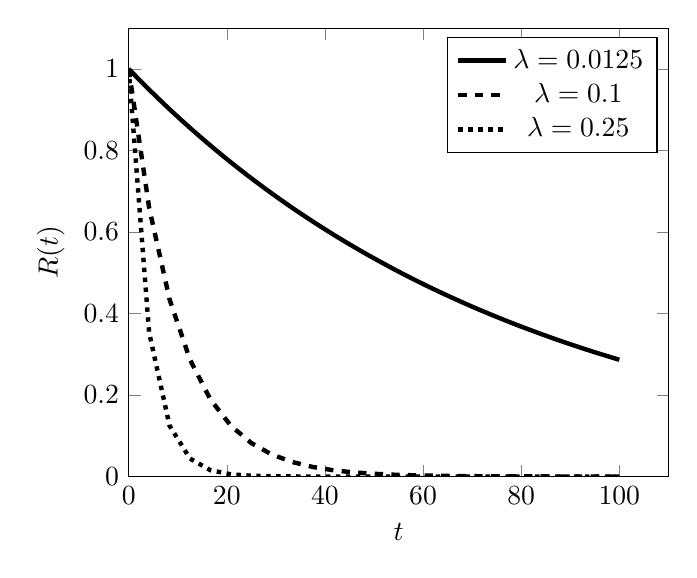
\begin{tikzpicture}
    \begin{axis}[
      scaled ticks=false,
      xmin=0,
      ymin=0,
      xlabel=$t$,
      ylabel=$R(t)$,
      ]
      \addplot[domain=0:100, black, ultra thick,smooth] {e^(-0.0125*x))};
      \addplot[domain=0:100, black, ultra thick,dashed] {e^(-0.1*x))};      
      \addplot[domain=0:100, black, ultra thick,dotted] {e^(-0.25*x))};
      \legend{$\lambda = 0.0125$, $\lambda=0.1$, $\lambda=0.25$}
    \end{axis}
  \end{tikzpicture}
  \caption{Reliability as a function of time}
  \label{fig:reliability}
\end{figure}

\subsection{Failure rate}

Assuming that a system on average will have $N_f$ failures, observed over a total time of $T_p$, we define the failure rate to be:
\begin{align}
  \lambda = \frac{N_f}{T_p}
\end{align}
Meaning that $\lambda$ has units of inverse time.

\begin{example}{Failure rate}{failure-rate}
  A system's manager recorded 1 failure in a 4 year period.
  What is the system's failure rate per year?
  \tcblower
  \begin{align}
    \lambda & = \frac{N_f}{T_p} \\
            & = \frac{1}{\SI{4}{\year}} \\
            & = \SI{0.25}{\per\year}
  \end{align}
\end{example}

\section{Bathtub curve}

In practice, the failure rate is elevated at the beginning and end of a system's life, following the so-called bathtub curve, \autoref{fig:bathtub-curve}.
The failure rate of any system normally excludes these particular periods and can be assumed to be constant for a particular system.

\autoimage{bathtub_curve}{Bathtub curve}{bathtub-curve}


\section{Mean time between failures}

The Mean Time Between Failures (MTBF) is a reciprocal of the failure rate, and has units of time:
\begin{align}
  \MTBF = \frac{1}{\lambda}
\end{align}

It is generally accepted that the mean time between failures relates only to the middle portion of the so-called ``bathtub curve'' of reliability, \autoref{fig:bathtub-curve}.

\begin{example}{Mean time between failures}{mtbf}
  A system on average fails on two occasions in five years.
  Calculate the mean time between failures.
  \tcblower
  \begin{align}
    \MTBF & = \frac{1}{\lambda} \\
          & = \frac{1}{\frac{N_f}{T_p}} \\
          & = \frac{T_p}{N_f} \\
          & = \frac{5}{2} \\
          & = \SI{2.5}{\year}
  \end{align}
\end{example}

\section{Mean time to repair}
Assuming that a failure has occured, it normally requires a repair time, during which the system is unavailable.
Averaged, we say that a particular type of failure has a Mean Time To Repair (MTTR).

\section{Inherent availability}
The inherent availability of a system tells us for what percentage of time it is likely to be available.
It is based on two ideas:
\begin{enumerate}
\item The system is available between failures, which should occur at intervals of the MTBF.
\item When a failure occurs, it will be unavailable for time taken to repair, ie the MTTR.
\end{enumerate}
So, the availability is essentially determined by how often a repair is needed and how long it takes.
Knowing the MTBF and MTTR, we can estimate the inherent availability, $A_i$ of a system:
\begin{align}
  A_i & = \frac{\MTBF}{\MTBF+\MTTR}
\end{align}
\begin{example}{Inherent availability}{inherent-availability}
  A system has an MTBF of 24 days and an MTTR of 12 hours.
  Calculate the inherent availability.
  \tcblower
  Assuming we take a base unit of days, so that 12 hours = 0.5 days.
  \begin{align}
    A_i & = \frac{24}{24 + 0.5} \\
        & = \SI{98}{\percent}
  \end{align}
\end{example}


\section{Operational availability}

The opearational availability of a system extends the inherent availability to incorporate scheduled maintenance downtime. 


%\chapter{Redundancy}
\label{ch:redundancy}

\section{N}

We say that to provide a particular function, we need a particular number of units $N$. 

\section{Common patterns}

\subsection{N+1}

If we need $N$ units, we add an additional unit to cover failures.
The additional unit is denoted $+1$.
This gives us the designation $N+1$.

\subsection{2N}

If we need $N$ units, we duplicate each individual unit giving us the designation $2N$.

Note that in practice sometimes the $2N$ and $N+1$ configurations lead to the same number of units, but usually one designation will be preferred over another to convey meaning. 

\end{document}






